\documentclass[tikz,border=5pt]{standalone}
\usetikzlibrary{calc}
\usetikzlibrary{decorations.pathmorphing}

\makeatletter

% gluon decoration (based on the original coil decoration)

\pgfdeclaredecoration{gluon}{coil}
{
  \state{coil}[switch if less than=%
    0.5\pgfdecorationsegmentlength+%>
    \pgfdecorationsegmentaspect\pgfdecorationsegmentamplitude+%
    \pgfdecorationsegmentaspect\pgfdecorationsegmentamplitude to last,
               width=+\pgfdecorationsegmentlength]
  {
    \pgfpathcurveto
    {\pgfpoint@oncoil{0    }{ 0.555}{1}}
    {\pgfpoint@oncoil{0.445}{ 1    }{2}}
    {\pgfpoint@oncoil{1    }{ 1    }{3}}
    \pgfpathcurveto
    {\pgfpoint@oncoil{1.555}{ 1    }{4}}
    {\pgfpoint@oncoil{2    }{ 0.555}{5}}
    {\pgfpoint@oncoil{2    }{ 0    }{6}}
    \pgfpathcurveto
    {\pgfpoint@oncoil{2    }{-0.555}{7}}
    {\pgfpoint@oncoil{1.555}{-1    }{8}}
    {\pgfpoint@oncoil{1    }{-1    }{9}}
    \pgfpathcurveto
    {\pgfpoint@oncoil{0.445}{-1    }{10}}
    {\pgfpoint@oncoil{0    }{-0.555}{11}}
    {\pgfpoint@oncoil{0    }{ 0    }{12}}
  }
  \state{last}[next state=final]
  {
    \pgfpathcurveto
    {\pgfpoint@oncoil{0    }{ 0.555}{1}}
    {\pgfpoint@oncoil{0.445}{ 1    }{2}}
    {\pgfpoint@oncoil{1    }{ 1    }{3}}
    \pgfpathcurveto
    {\pgfpoint@oncoil{1.555}{ 1    }{4}}
    {\pgfpoint@oncoil{2    }{ 0.555}{5}}
    {\pgfpoint@oncoil{2    }{ 0    }{6}}
  }
  \state{final}{}
}

\def\pgfpoint@oncoil#1#2#3{%
  \pgf@x=#1\pgfdecorationsegmentamplitude%
  \pgf@x=\pgfdecorationsegmentaspect\pgf@x%
  \pgf@y=#2\pgfdecorationsegmentamplitude%
  \pgf@xa=0.083333333333\pgfdecorationsegmentlength%
  \advance\pgf@x by#3\pgf@xa%
}

\makeatother
\begin{document}
  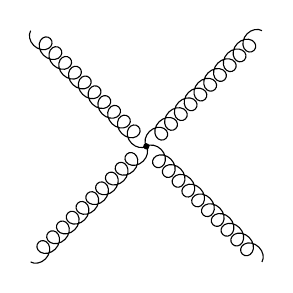
\begin{tikzpicture}
        \fill (0,0) circle (0.04cm);
        \path (0,0) edge[decorate,decoration={gluon, amplitude=3.0pt, segment length=5pt, aspect=1.1}] (1.4,1.4);
        \path (0,0) edge[decorate,decoration={gluon, amplitude=3.0pt, segment length=5pt, aspect=1.1}] (1.4,-1.4);
        \path (0,0) edge[decorate,decoration={gluon, amplitude=3.0pt, segment length=5pt, aspect=1.1}] (-1.4,-1.4);
        \path (0,0) edge[decorate,decoration={gluon, amplitude=3.0pt, segment length=5pt, aspect=1.1}] (-1.4,1.4);
  \end{tikzpicture}
\end{document}
